\documentclass[10pt,a4paper]{report}
\usepackage[a4paper, total={6in, 8in}]{geometry}
\usepackage[utf8]{inputenc}
\usepackage{amsmath}
\usepackage{amsfonts}
\usepackage{amssymb}
\usepackage{graphicx}

\begin{document}

{\LARGE \center Advanced Computer Graphics \\ Homework 6\\ Particle System Part 2\\}
{\large \center Group 8\\ Damien Doy - 244206\\
Jason Racine - 244270\\
Alexandre Veuthey - 224295\\
}

\section*{Computation of the triangle area forces}
In order to find the force at each vertice of the triangle we have to find the following partial derivative (as stated in the lecture):\\
$F_i=-\frac{\partial EA(x_0,x_1,x_2)}{\partial x_si}$ 
where 
$EA(x_0,x_1,x_2)=0.5k_A(area(x_0,x_1,x_2)-A)^2$\\
and \\
$area(x_0,x_1,x_2)=0.5((x_1.x-x_0.x)(x_2.y-x_0.y)-(x_2.x-x_0.x)(x_1.y-x_0.y))$\\
By solving these equations, we get:\\\\
$Fi=-\frac{\partial EA(x_0,x_1,x_2)}{\partial x_i}=k_A(area(x_0,x_1,x_2)-A)
\frac {\partial area(x0,x1,x2)}{\partial x_i}$\\\\
And by solving the partial derivative we get the following forces for each particles:\\\\
$F_0=-0.5dEA(x_{y1}-x_{y2}, x_{x2}-x_{x1})\\
F_1=-0.5dEA(x_{y2}-x_{y0}, x_{x0}-x_{x2})\\
F_2=-0.5dEA(x_{y0}-x_{y1}, x_{x1}-x_{x0})\\
$where $dEA=k_A(area(x_0,x_1,x_2)-A)$

\section*{Computation of the Jacobian}

\subsection*{Gravity}
Let's begin with the gravitation force, which is defined as\\
$
F_G=\begin{pmatrix}
0 \\
-Gm \\
\end{pmatrix}
$\\
Since the force of gravity does not depend on the position of the particle, the 2x2 Jacobian
of this force by the particle position is a null matrix and doesn't have to be added to the solver\\
\subsection*{Centre force}
The center force is defined as:\\
$
F_C=\begin{pmatrix}
-Cx\\
-Cy\\
\end{pmatrix}
$\\
And thus, the jacobian of this force is:\\
$
J_C=\begin{pmatrix}
-C && 0\\
0 && -C\\
\end{pmatrix}
$\\
\subsection*{Force-based collisions}
The force based collision is applied to the particle only when\\
$xn_x+yn_y+n_z-p_{radius} < 0$ where $x$ and $y$ are the position of the particle, and $n_x$, $n_y$ and $n_z$ are the parameters of the line equation. Then the force is:\\
$
F_{Col}=\begin{pmatrix}
-n_x(xn_x+yn_y+n_z-p_{radius})k_{col}\\
-n_y(xn_x+yn_y+n_z-p_{radius})k_{col}
\end{pmatrix}
=
\begin{pmatrix}
-k_{col}(xn_x^2+yn_xn_y+n_xn_z-p_{radius}n_x)\\
-k_{col}(xn_xn_y+yn_y^2+n_yn_z-p_{radius}n_y)
\end{pmatrix}
$\\\\
Then the jacobian is\\\\
$
J_{Col}=\begin{pmatrix}
-k_{col}n_x^2 	&& -k_{col}n_xn_y\\
-k_{col}n_xn_y 	&& -k_{col}n_y^2
\end{pmatrix}
$
\subsection*{Damped-spring forces}
Forces are:\\\\
$
F_{spring0}=-\begin{pmatrix}
(k_s + k_d) \frac{p_{x0}-p_{x1}}{||p_0-p_1||}\\
(k_s + k_d) \frac{p_{y0}-p_{y1}}{||p_0-p_1||}\\
\end{pmatrix}
$\\\\
For the particle $p_0$ with force $F_{spring0}$, the jacobian is\\\\
$
J_{spring0}=\begin{pmatrix}
-(k_s+k_d)(\frac{(x_1-x_0) len'+len}{len^2}) 	&& (k_s+k_d)(\frac{(x_0-x_1) len'}{len^2})\\
(k_s+k_d)(\frac{(y_0-y_1) len'}{len^2}) 	&& -(k_s+k_d)(\frac{(y_1-y_0) len'+len}{len^2})\\
\end{pmatrix}
$\\\\
This is only one of the 4 jacobian we have to calculate in order to have this force.\\
The final jacobian will be a 4x4 matrix.
\subsection*{Area preservation forces}
The force is defined as:\\\\
$
F_{area0}=-0.5dEA\begin{pmatrix}
p_{y1}-p_{y2}\\
p_{x2}-p_{x1}
\end{pmatrix}
$\\\\
This will give a 3x3 sparse jacobian where:\\\\
$\frac{\partial F_{area0}}{\partial p_{y1}} = -0.5dEA$\\\\
$\frac{\partial F_{area0}}{\partial p_{x0}} = 0$

\section*{Computation of the equilibrium force}
In order to distribute the particles on the screen, we added a force that acts on every particles. They repulses themselves like same polarity charges in electromagnetism.\\
To avoid a unstable system and to reduce the computation time, we limited this force to a certain radius around each particle. This radius is equals to\\
$radius = C(\frac{1}{dist}-1)*normal_{p_0,p_1}$ where $dist \in {0, 1}$ is the distance between two particles normalized. $C$ is a constant that makes the equilibrium force stronger or weaker.\\
Here is a graph of this function:\\
\begin{center}
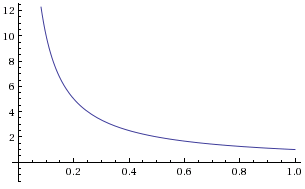
\includegraphics[scale=0.5]{graph_equib.png}\\
\end{center}
The advantage of a strong force, is that particles will distribute uniformly faster, but a great force will make the system go unstable.\\
A weak force can also be advantageous, particles will move slower to their positions but there is less risk of particles flying off.\\
Here we tested the equilibrium force on 30, 100, 250 particles, with verlet integration and impulse based forces:\\
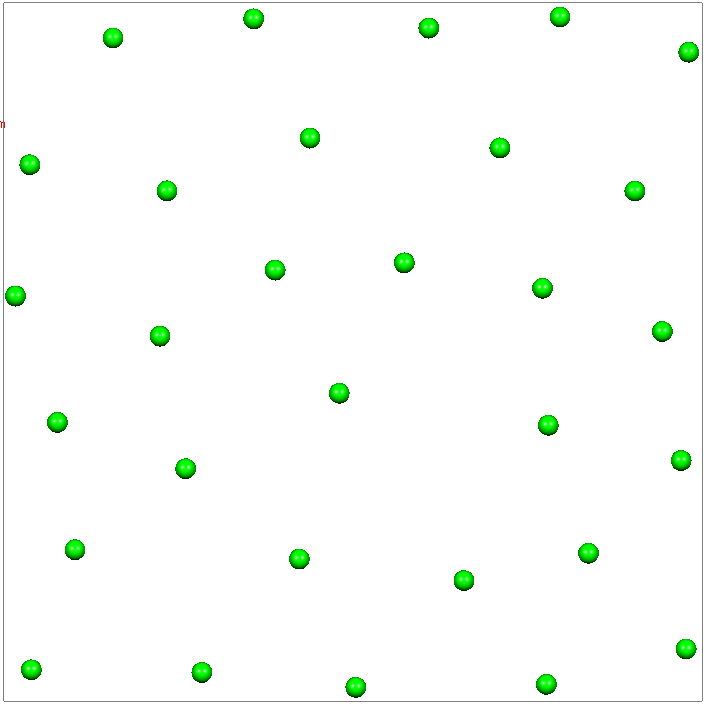
\includegraphics[scale=0.25]{30.png}
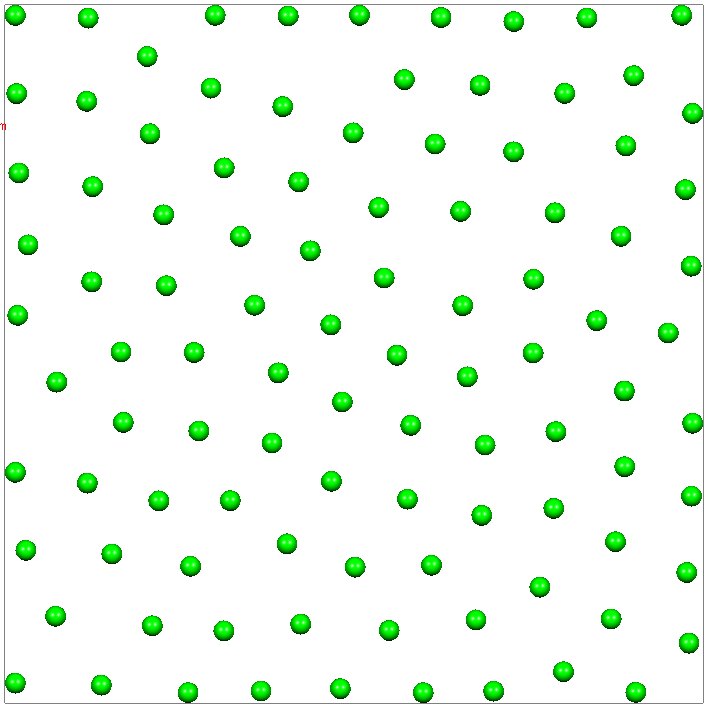
\includegraphics[scale=0.25]{100.png}\\
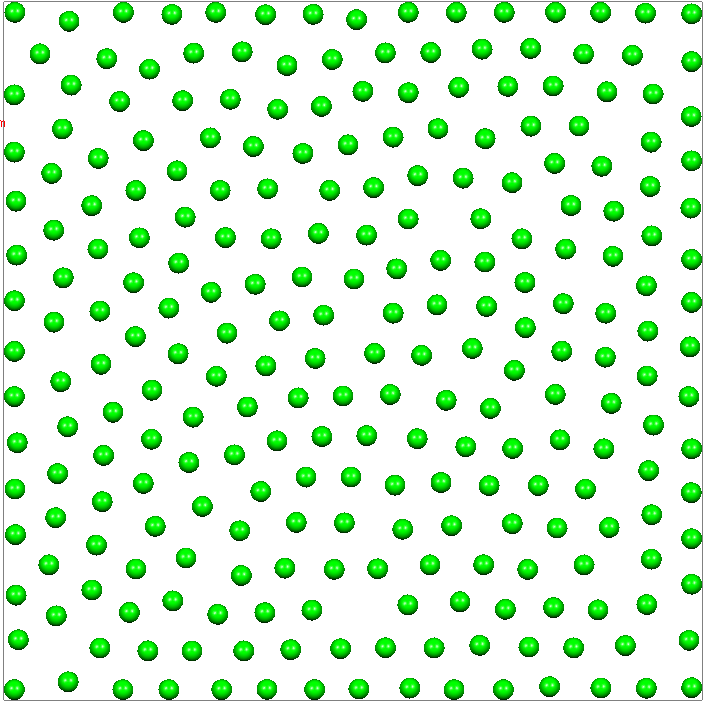
\includegraphics[scale=0.25]{250.png}

\section*{Comparison of the integration methods}
The verlet integration is the most stable of the integrations methods in this lab.\\
The euler integration method is really unstable and particles will rarely find a rest point (they will bounce around or jiggle when there are springs). The system can go unstable very easily with springs. A lower timestep will solve this problem at the cost of computation time.\\
The midpoint integration method have the same problems as euler but the instabilites are reduced for the same time stamp.\\
In the case of euler and midpoint integration, all inacurracies and the unstability of the system can be solved by reducing the timestamp.\\
The verlet integration is the most stable. For the same timestamp as used for euler and midpoint, particles will find a rest point at some point and the scene with the octogon will stay stable, even if violent forces are acting on the shape. The verlet integration can be even used with larger timestamps, the system will stay stable at dt=0.002 and will show some problems at dt=0.004.\\
In the case of implicit euler, the same problems as explicit euler appear. That is, the system go unstable when the timestamp is too high. A lower time stamp (t=0.00025) solve the problem.
\end{document}